%!TEX root = ./Thesis.tex

\chapter{Vector vortex beam recognition}
\label{Section:ML_VVBs}


\textit{Introduction--} Light is endowed with~\ac{OAM}~\cite{allen1992orbital,padgett2004lights}, a degree of freedom associated with structured (i.e. non-plane) wavefronts and characterized by an azimuthal phase dependence. 
When such phase dependence is coupled with a helicoidal transverse profile of the polarization, one has a \ac{VVB}~\cite{erhard2017twisted,padgett2004lights}.
The interest in such beams is motivated by the multiple applications in different fields of classical and quantum optics \cite{marrucci2011spintoorbital}: from particle trapping to metrological applications in microscopy~\cite{cardano2015spin–orbit, rubinsztein-dunlop2016roadmap} and for \ac{OAM}-based communications schemes in free-space and in-fibre \cite{willner2015optical,cozzolino2019aircore}.
\acp{VVB} are also often employed in quantum information protocols due to the correlations between polarization and spatial modes of single photons. Photonic platforms for quantum sensing and metrology operated through information-encoding in such DoF have been reported~\cite{fickler2012quantum,dambrosio2013photonic}. OAM-based schemes for investigating fundamentals of quantum mechanics \cite{goswami2018indefinite}, for quantum communication and cryptography \cite{vallone2014freespace,wang2015quantum,mirhosseini2015highdimensional,malik2016multiphoton,sit2017highdimensional,cozzolino2019orbital} quantum walks~\cite{zhang2010implementation,goyal2013implementing,cardano2015quantum}, quantum simulation~\cite{cardano2016statistical,cardano2017detection}, and quantum state engineering~\cite{innocenti2017quantum,giordani2019experimental} have been demonstrated. 

Despite the potential that \acp{VVB} have in several areas, many questions regarding decoding the information in both OAM and polarization are still open. Various techniques of OAM-demultiplexing envisage the need of additional instruments -- such as interferometry~\cite{leach2002measuring,slussarenko2010polarizing,bauer2013nanointerferometric} or spatial filtering \cite{berkhout2010efficient,bolduc2013exact,malik2014direct}
-- to be efficiently implemented. These introduce detrimental effects of loss and noise~\cite{qassim2014limitations}. Moreover, the challenge of performing state tomography in such high-dimensional framework, a fundamental task in quantum information processing~\cite{paris2004quantum,banaszek2013focus}, can hardly be overestimated. The design and demonstration of reliable techniques for the generation and classification of~\acp{VVB} is thus highly desirable. Indeed 
substantive efforts on finding novel platforms are subject of intense research activities~\cite{liu2016generation,ndagano2017creation,cardano2015spin–orbit,rubinsztein-dunlop2016roadmap},
as proved, for example, by the ultimate results for VVBs synthesis  in integrated photonics~\cite{chen2018mapping,cai2012integrated,liu2017direct} and generation by plasmonic metasurfaces~\cite{karimi2014generating,yue2016vector} 
.


 Recently,~\ac{ML} techniques have emerged as versatile tools to tackle a variety of tasks in experimental platforms, and have been proven useful, in particular, to improve the characterization of quantum protocols and dynamics ~\cite{carrasquilla2019reconstructing,giordani2018experimental,agresti2019pattern,lumino2018experimental,rocchetto2019experimental,butler2018machine,fischer2006predicting,melnikov2018active,wang2017experimental}.
In the context of structured light, %in classical and quantum optics, 
neural networks (NN) have been used to classify \ac{OAM} states of classical light for long distance free-space communication purposes, even in the presence of environmental turbulence~\cite{krenn2014communication,krenn2016twisted,doster2017machine,
park2018demultiplexing, lohani2018turbulence, li2018joint}.
In this paper, we apply \ac{ML} to classify and characterize experimental \ac{VVB} states generated using a platform inspired  to photonics \acp{QW} in the \ac{OAM} and polarization DoFs~\cite{innocenti2017quantum,giordani2019experimental}. {Our approach requires neither additional interferometry stabilization nor spatial filtering, thus providing a robust strategy to decode the information stored in \acp{VVB} and a promising pathway to the management of higher dimensional quantum systems}. 

Our \ac{ML} approach leverages both supervised and unsupervised techniques: we  train a \ac{CNN} to classify experimental images belonging to one of a number of predefined classes of states. This method gives good prediction accuracy, while remaining fairly problem-agnostic and thus useful for diverse applications. However, while providing high prediction accuracy, NN-based methods are typically of difficult interpretation, which cast doubts on the trustfulness of the results obtained through them. We thus employ an alternative method -- based on the joint application of dimensionality reduction (DR) via \ac{PCA} and classification via \ac{SVM} -- to categorize experimental images. While significantly easier to interpret, this method gives comparable results to \acp{CNN}.

By comparing the performances of such \ac{ML} techniques, we show their reliability for the classification of~\ac{VVB} states. Moreover, we show how linear DR can be used to infer properties about the geometric structure of the set of quantum states corresponding to a given set of experimental images.
Our findings demonstrate the reliability of \ac{ML} methods as building blocks for automatized quantum information protocols over high-dimensional systems. 

Our work makes significant steps forward  with respect to previous endeavours: while Refs.~\cite{krenn2014communication,krenn2016twisted,doster2017machine, park2018demultiplexing, lohani2018turbulence, li2018joint} leverage NN to process OAM states, we work on VVBs, that is states in which OAM is intertwined with polarization. Moreover, the class of problems that we are able to address through the variety of ML techniques deployed here allows us to tackle both classification and regression tasks, thus enabling the reconstruction of the input states in relevant cases that we address explicitly.


\begin{figure}[t]
	\centering
    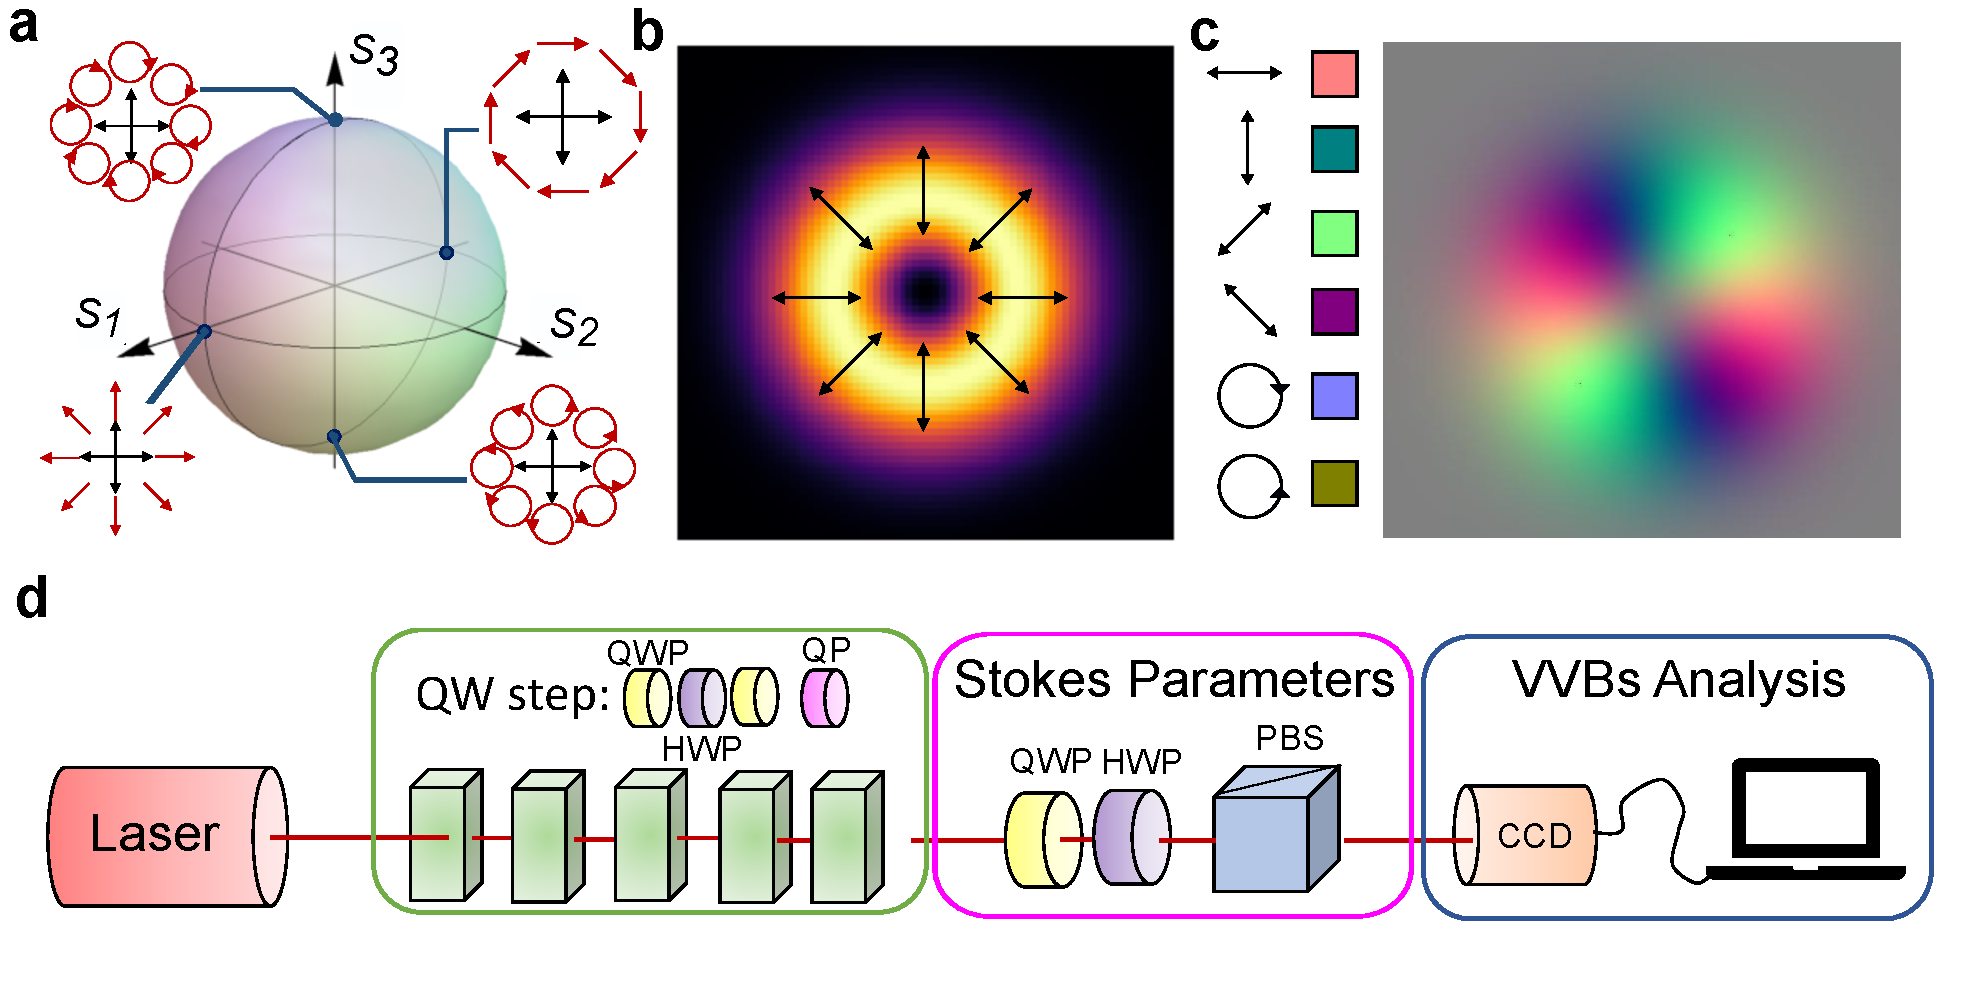
\includegraphics[width=\textwidth]{Figures/quantum-walks/VVBs-VVBschemaQW.pdf}
    \caption{
    	\textbf{Vector vortex beams: representation and generation.}
		\textbf{\emph{(a)}}
		Poincar\'e sphere representation for $|m_{1,2}|=1$. Each point on the sphere surface corresponds to specific polarization patterns. 
		%\textcolour{orange}{Radial and azimuthal \ac{VVB}s correspond to $\theta=\frac{\pi}{2}$, $\phi=0$ and $\frac{\pi}{2}$ respectively.} 
		\textbf{\emph{(b)}}
		A radially polarized \ac{VVB}: at a given point in the trasversal plane the polarization vector has a different orientation. The Stokes parameters vary accordingly in the plane.
		\textbf{\emph{(c)}}
		Colour encoding of the polarization pattern. 
		The legend reports the correspondence between colours and the various polarizations.
		On the right we have the resulting colour pattern for the VVB in panel {\bf b}. Grey colour 
		corresponds to unpolarized light.
		\textbf{\emph{(d)}}
		Experimental apparatus for the generation of \acp{VVB}. A cw laser emits a Gaussian beam $\on{TEM}_{00}$ at $808$ nm. Light undergoes a 5-step quantum walk realized through a sequence of waveplates and q-plates. 
		A CCD camera-based detection stage acquires information on the Stokes parameters and the polarization pattern. Based on the intensity measured at each pixels of the  camera, Stokes parameters are evaluated and converted into RGB-coloured pictures.
	}
\label{fig:qw_poinc_sphere}
\end{figure}

\begin{figure}
	\centering
	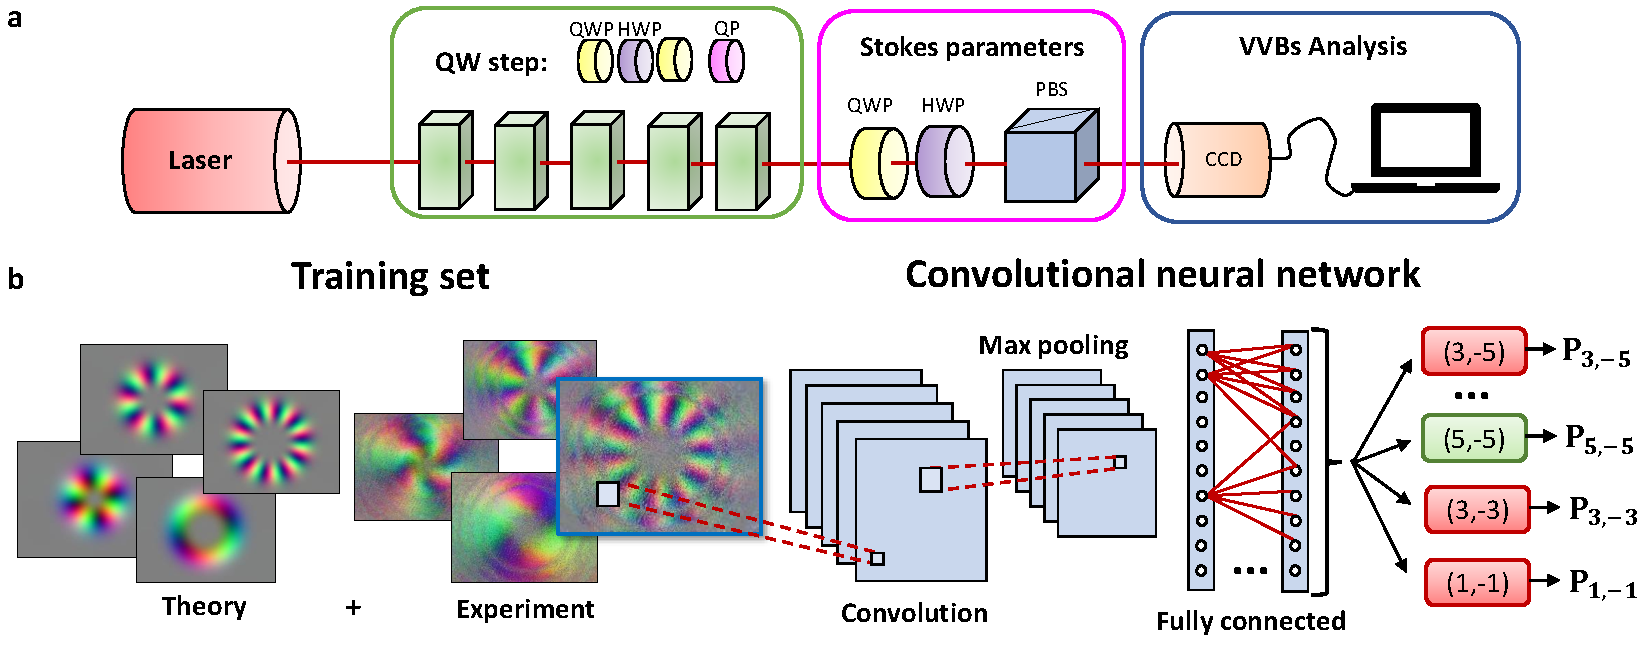
\includegraphics[width=\textwidth]{Figures/quantum-walks/VVBs-schema.pdf}
\end{figure}

\begin{figure}
	\centering
	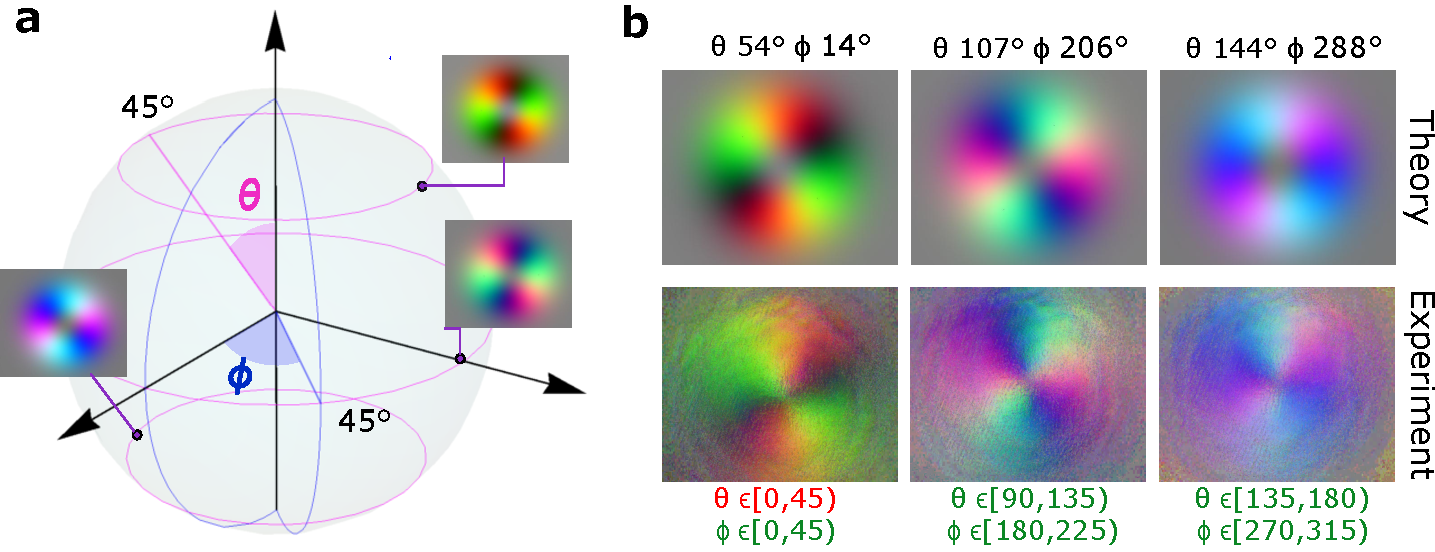
\includegraphics[width=\textwidth]{Figures/quantum-walks/VVBs-results_th_ph_old.pdf}
	\caption{
		\textbf{Training set on high-order Poincar\'e sphere.}
		\textbf{\emph{(a)}} Poincar\'e sphere for \acp{VVB} with $|m_{1,2}|=1$.
		Magenta-coloured parallels (Blue-coloured meridians) mark intervals between consecutive values of $\theta$ ($\phi$). 
	    Along a meridian the colours of the pattern vary from the hottest to the coldest ones. Along a parallel the pattern rotates. 
	    \textbf{(b)} Comparison between experimental \ac{VVB} with the expected picture for $(\theta, \phi)$ reported below.
	}
\end{figure}


\textit{Experimental generation of Vector Vortex Beams--} 
Light carrying non-zero~\ac{OAM} is commonly described using Laguerre-Gauss (\ac{LG}) modes.
These are solutions of the Helmholtz equation in the paraxial approximation, and are characterized by two integer numbers $(m, p)$, the former describing the azimuthal phase structure of the beam, and the latter describing its radial intensity profile.
Each~\ac{LG} mode carries a set amount of angular momentum, which in the single-photon regime equals $\hbar m$~\cite{allen1992orbital}.
\acp{VVB} can be obtained by superposing orthogonal polarizations to \ac{LG} modes \cite{padgett2004lights}. 
The electric field $\Vec{E}_{m_1m_2p}$ of a \ac{VVB} mode can be decomposed into the coherent superposition of~\ac{LG} modes with same $p$ and azimuthal numbers $m_1>m_2$ carried by orthogonal polarizations, that is
$    \Vec{E}_{m_1m_2p}=\Vec{e}_L \cos{ \frac{\theta}{2}}\text{ LG$_{m_1p}$} +\Vec{e}_R e^{i \phi} \sin{ \frac{\theta}{2}}\text{ LG$_{m_2p}$}$,
where $\theta\in[0,\pi], \phi\in[0,2\pi]$ and the unit vectors $\Vec{e}_{L,R}$ stand for left and right circular polarization, respectively.
For the purpose of this work it is possible to ignore the radial number, setting $p=0$. For any given value of the set of parameters $(m_1$, $m_2, \theta, \phi)$  the polarization pattern of a \acp{VVB} can be mapped onto a generalized Poincar\'e sphere~\cite{milione2011higherorder} [cf. Fig.~\ref{fig:qw_poinc_sphere}], and 
it can thus be reconstructed by measuring the values taken by the Stokes parameters $S_{j}~(j=1,2,3)$, which are obtained by projecting the state of the field onto the polarization basis $\{b_1,b_2,b_3\}$ with $b_1=( H,V )$, $b_2=( D,A )$, $b_3=( L,R )$ as 
    $    S_{b_j}=(I_{b_j,1}-I_{b_j,2})/(I_{b_j,1}+I_{b_j,2})~~(j=1,2,3)$.
Here $I_{b_j,k}$ stands for the intensity corresponding to one of the polarization states $H,V,D,A,L,R$.

For a \ac{VVB}, the values of $S_j$ depend on the coordinates $x$ and $y$ in the transverse propagation plane \cite{cardano2012polarization}.
To visually represent the polarization patterns of \acp{VVB}, we use a RGB colour encoding in which the values of $S_j$ are interpreted as strengths of the corresponding colour. In Fig.~\ref{fig:qw_poinc_sphere}b and c we report an example of such colour-map for radially polarized \ac{VVB}. A natural way to generate~\acp{VVB} is using \emph{q-plates}~\cite{marrucci2006optical,cardano2012polarization}, which are inhomogenous birefringent plates modifying the OAM of the incoming light conditionally on its polarization 
%\rmv{as $\Vec{e}_L \text{ LG}_m {\rightarrow} \Vec{e}_R\text{ LG}_{m+2q}$, $\Vec{e}_R \text{ LG}_m{\rightarrow} \Vec{e}_L\text{ LG}_{m-2q}$.
%Here, $q\in\mathbb{Z}$ is the charge of the topological singularity located at the center of the q-plate}~\cite{marrucci2006optical,cardano2012polarization}. 



Our scheme for generating \ac{VVB} states is based on the dynamics set by a discrete-time QW in the OAM DoF, where the order of \ac{LG} modes is increased or decreased according to the polarization state, which embodies the coin of the walk~\cite{zhang2010implementation,goyal2013implementing,cardano2015quantum,innocenti2017quantum,giordani2019experimental}. 
\ac{VVB}s are generated via a sequence of waveplates -- to control polarization -- interspersing 5 cascaded q-plates (cf. Fig.~\ref{fig:qw_poinc_sphere}d). This allows for the generation of different classes of VVB states whose {OAM quantum number} takes odd values in the interval $\{-5,..,5\}$.
We then collect images associated with different polarization states and use them to train and benchmark our \ac{ML}-based approaches to classification, as discussed in the next section. 

\begin{figure}[b]
    \centering
    % \includegraphics[width=\columnwidth]{Fig2.pdf}
    \caption{
    {\bf a,} 
    Working principles of the \ac{CNN}. The training set consists of a series of computer-generated pictures and others collected from the experimental platform.
    {\bf b,} 
    Scheme to classify experimental \ac{VVB} images. First, the dimension of the dataset is reduced via linear PCA. Then, a SVM classifier is trained over 
    such reduced representation 
    to predict the classes of future images of \ac{VVB}s. {\bf c,} principal components obtained using \ac{PCA} on simulated datasets of noisy \acp{VVB}. The first (second) row shows the first seven principal components obtained on the dataset $\mathcal S_1$ ($\mathcal S_2$). 
    The first 6 (all 7) components correspond to non-vanishing singular values. 
    }
    \label{fig:class_techniques}
\end{figure}



\begin{figure}
    \centering
    \includegraphics[width=\textwidth]{Figures/quantum-walks/VVBs-cnn+result.pdf}
    \caption{
	    \textbf{\emph{Convolutional Neural Network (CNN) results.}}
	    \textbf{(a)} Comparison between expected and recorded polarization patterns for some \ac{VVB}s of the ensemble in table, with the corresponding values $(m_1,m_2)$. 
	    %and the recognition accuracy by the network, averaged on $100$ experimental pictures, not included in the training and validation sets, per each class, for two cases. In magenta the resulting accuracy with a training set made by theoretical images and a validation set composed only of experimental pictures. 
	    %In blue the results with the same validation test and a fraction $N_{exp}/N_{th}=0.125$ of experimental VVBs in the training set. 
	    {\bf b,} scaling of the mean accuracy per class, obtained for discerning $(m_1, m_2)$ in the 15 \ac{VVB}s classes,
	    %for the demultiplexing of OAM components for the 15 \ac{VVB}s, %\st{that can be generated with a 5-step quantum walk}, 
	    against the fraction of experimental pictures in the training set. 
	    %The arrows mark the points corresponding to the accuracy %in panel {\bf a}. 
	    Inset: best true-table. %$\mathcal{M}$
	    %\textcolour{orange}{corresponding to the blue arrow}.  %\st{Labels in the} 
	    Rows (columns) stand for the possible $(m_1,m_2)$ pairs (as assigned by the CNN). The matrix elements have been averaged over $100$ experimental images per class. 
	    %The mean accuracy per class $\mathcal{A}$, defined as the trace of $\mathcal{M}$ divided per the number of classes, is $0.989$.
    }
    \label{fig:resultsCNN}
\end{figure}

%\begin{figure*}[t]
%    \includegraphics[width=\textwidth]{Fig2.pdf}
%    \caption{ \textbf{Convolutional Neural Network %(CNN) results. a,} conceptual depiction of the %working principles of the network. The %training set consists of a series of %computer-generated pictures and others %collected from the experimental platform. The %\ac{CNN} is made by a series of convolutional %and max-pooling layers, ended with a fully %connected layer. After the training stage the %network is able to classify the pictures %recorded in the experiment. {\bf b,} %comparison between expected and recorded %polarization patterns for some \ac{VVB}s of %the ensemble. Below picture the corresponding %values $(m_1,m_2)$ and the recognition %accuracy by the network, averaged on $100$ %experimental picture, not included in the %training and validation sets, per each class, %for two cases. In magenta we report the %resulting accuracy with a training set made by %theoretical images and with a validation set %composed only by experimental pictures. In %blue the results with the same validation test %and a fraction $N_{exp}/N_{th}=0.125$ of %experimental VVBs in the training set. {\bf %c,} the best true-table $\mathcal{M}$, %corresponding to the blue results in {\bf b}, %obtained for the demultiplexing of OAM %components for the 15 \ac{VVB}s that can be %generated with a 5-step quantum walk. Labels %in the rows (columns) stand for the possible %pairs of values $(m_1,m_2)$ (the values %assigned by the CNN). The elements of the %matrix have been averaged over $100$ %experimental images for each class. The mean %accuracy per class $\mathcal{A}$, defined as %the trace of $\mathcal{M}$ divided per the %number of classes, amounts to $0.989$. {\bf %d,} scaling of the mean accuracy per class %against the fraction of experimental pictures %in the training set. The points marked with an %arrow correspond to the accuracy reported in %panel \textbf{b}.}
%    \label{fig:resultsCNN}
%\end{figure*}


\textit{Classification via Convolutional Neural Networks--} We start by training a \ac{CNN} so as to retrieve the values of $m_{1,2}$ in a given VVB state through the experimental values of the Stokes parameters resulting from polarization measurements.  \acp{CNN} build a class of translation-invariant deep neural networks suited for image classification
. This feature makes them well-suited to recognize off-center images, 
 for segmented handwritten digits \cite{simard2003best,ciresan2011flexible} 
 and facial expressions recognition \cite{matsugu2003subject}. 
 Their operations are based on a features extractor and a classifier. The former consists of convolutional and max-pooling layers, while the latter is a fully connected layer which performs non-linear transformations of the extracted features and determines which of them is most correlated to a particular class.
 
The network is trained firstly with training and test sets consisting of simulated images of the \ac{VVB}s achievable by a 5-step quantum walk. The task is then to discern between $15$ classes. For each class in which $m_1 < m_2$, we have generated   states with $\theta=\pi/2$ and $\phi$ varying from $0$ to $2 \pi$. The size of the training set is $400$ images per class and $100$ for the test set. In these conditions, the network achieves an accuracy of $100\%$ when tested with theoretical images. 
We have then collected $100$ images for each class from the experimental quantum walk apparatus and used this sample as a validation test for the network [cf. Fig.~\ref{fig:class_techniques}a]. Fig.~\ref{fig:resultsCNN}a-b shows the mean accuracy per class against the fraction of experimental pictures in the training set, starting from one consisting of computer-generated images only.
Remarkably, a small increase of the number of experimental pictures in the training set results in a good accuracy reached by the network [cf. Fig.~\ref{fig:resultsCNN}b]: when only $12.5\%$ of experimental images are used, an average accuracy of $\sim 0.989$ is found.
%, as reported in Fig.~\ref{fig:resultsCNN}c. 


%\begin{figure}[t]
%    \includegraphics[width=\columnwidth]{Fig3.pdf}
%    \caption{\textbf{%Training set on high-order Poincar\'e %sphere. 
%    a,} Poincar\'e sphere for \ac{VVB}s with $|m_{1,2}|=1$. %Magenta-coloured parallels (Blue-coloured meridians) mark %intervals between consecutive values of $\theta$ ($\phi$). 
%    %(only the first two meridians are shown)
%    %We report some \ac{VVB}s: 
%    Along a meridian the colours of the pattern vary from the %hottest to the coldest ones. Along a parallel the pattern %rotates. 
%    {\bf b,} Comparison between experimental \ac{VVB} with the %expected picture for $(\theta, \phi)$ reported below.}
%    \label{fig:results_qubit}
%\end{figure}


The same apparatus allows to retrieve the values $(\theta,\phi)$ for a fixed $(m_1, m_2)$,
%The problem is analogous to that of state tomography.%, which is a crucial primitive in quantum information. 
%\rmv{. by suitable measurements on polarization and OAM DoFs
%We  perform a complete set of polarization measurements (projecting onto a set of mutually unbiased %basis), followed by the recording of the intensity distribution of the beam in the transverse plane. %Such measurement stage allows for a full reconstruction of the VVBs states}
providing enough information about the coordinates on the Poincar\'e sphere. We then test the performance of the CNN in the classification of each recorded \ac{VVB} according to the values $(\theta,\phi)$ for $|m_{1,2}|=1$. To do this, the network should discriminate rotations in the polarization patterns (i.e. changes in $\phi$) and variations in the colour tone (i.e. changes in $\theta$). However a drawback of using CNN is that \ac{VVB}s with $|m_i|\gg1$ display a polarization pattern whose periodicity decreases as $\frac{2\pi}{|m_1-m_2|}$ (cf. Fig.~\ref{fig:resultsCNN}a)~ \cite{fickler2012quantum,dambrosio2013photonic}. This complicates the recognition of $\phi$ value as changes in the phase generate only small rotations of the pattern. Furthermore, the classification of the VVB on the sphere requires a discretization of  $\theta$ and $\phi$, which results in dividing the sphere in sectors. This means that VVBs placed at the borders of these intervals are more difficult to assign to a specific class.

The network is then trained with ideal patterns for different positions on the sphere. The latter is divided in sectors covering intervals in which $\theta$ and $\phi$ vary in steps of $\pi/4$ (see Fig.~\ref{fig:PCAresults}a). The resulting number of classes is $26$: 8 sectors for $\phi$ and 3 for $\theta$. In addition, there are 
2 classes for the poles where $\phi$ is undetermined. We have trained the CNN with 500 images per class in the training set and 125 in each class of the test set. The maximum accuracy reached is $\sim 0.90$. The main reason of such result, which is inferior with respect to the problem of only inferring $m_{1,2}$, is that here we had to artificially coarse-grain two continuous parameters. 
%In the next section we show how a PCA-based approach can help to improve the performance for this classification task.



\textit{Dimensionality reduction--} High-dimensional dataset can often be effectively represented using a smaller number of dimensions -- while preserving the important information of the original dataset -- using a DR approach~\cite{cord2008machine,fodor2002survey}. This has several advantages, from easing data visualisation, to improving the efficiency of classification and regression algorithms, which can be used on the reduced representation of the data. %Dimensionality reduction can also be useful to reduce the overfitting in a classifier, weeding out redundant and unnecessary information.
A common method to perform linear DR is \ac{PCA}, which finds the set of orthogonal directions in the high-dimensional feature space that optimally capture the information in the dataset. Specifically, \ac{PCA} finds the directions projecting the dataset onto which gives the greatest possible variance.

While DR has been fruitfully applied to various types of datasets, we have strong arguments suggesting that \emph{linear} DR is well suited to our needs.
In fact, the linearity of the mapping sending each state to the associated set of detection probabilities implies that the geometrical features of the set of quantum states are transferred to the set of vectorised experimental intensity images. Using {linear} DR, we can thus recover the directions in the space of experimental images corresponding to directions in the underlying state space (cf. \cite{SI}).

\begin{figure}[t]
	\centering
	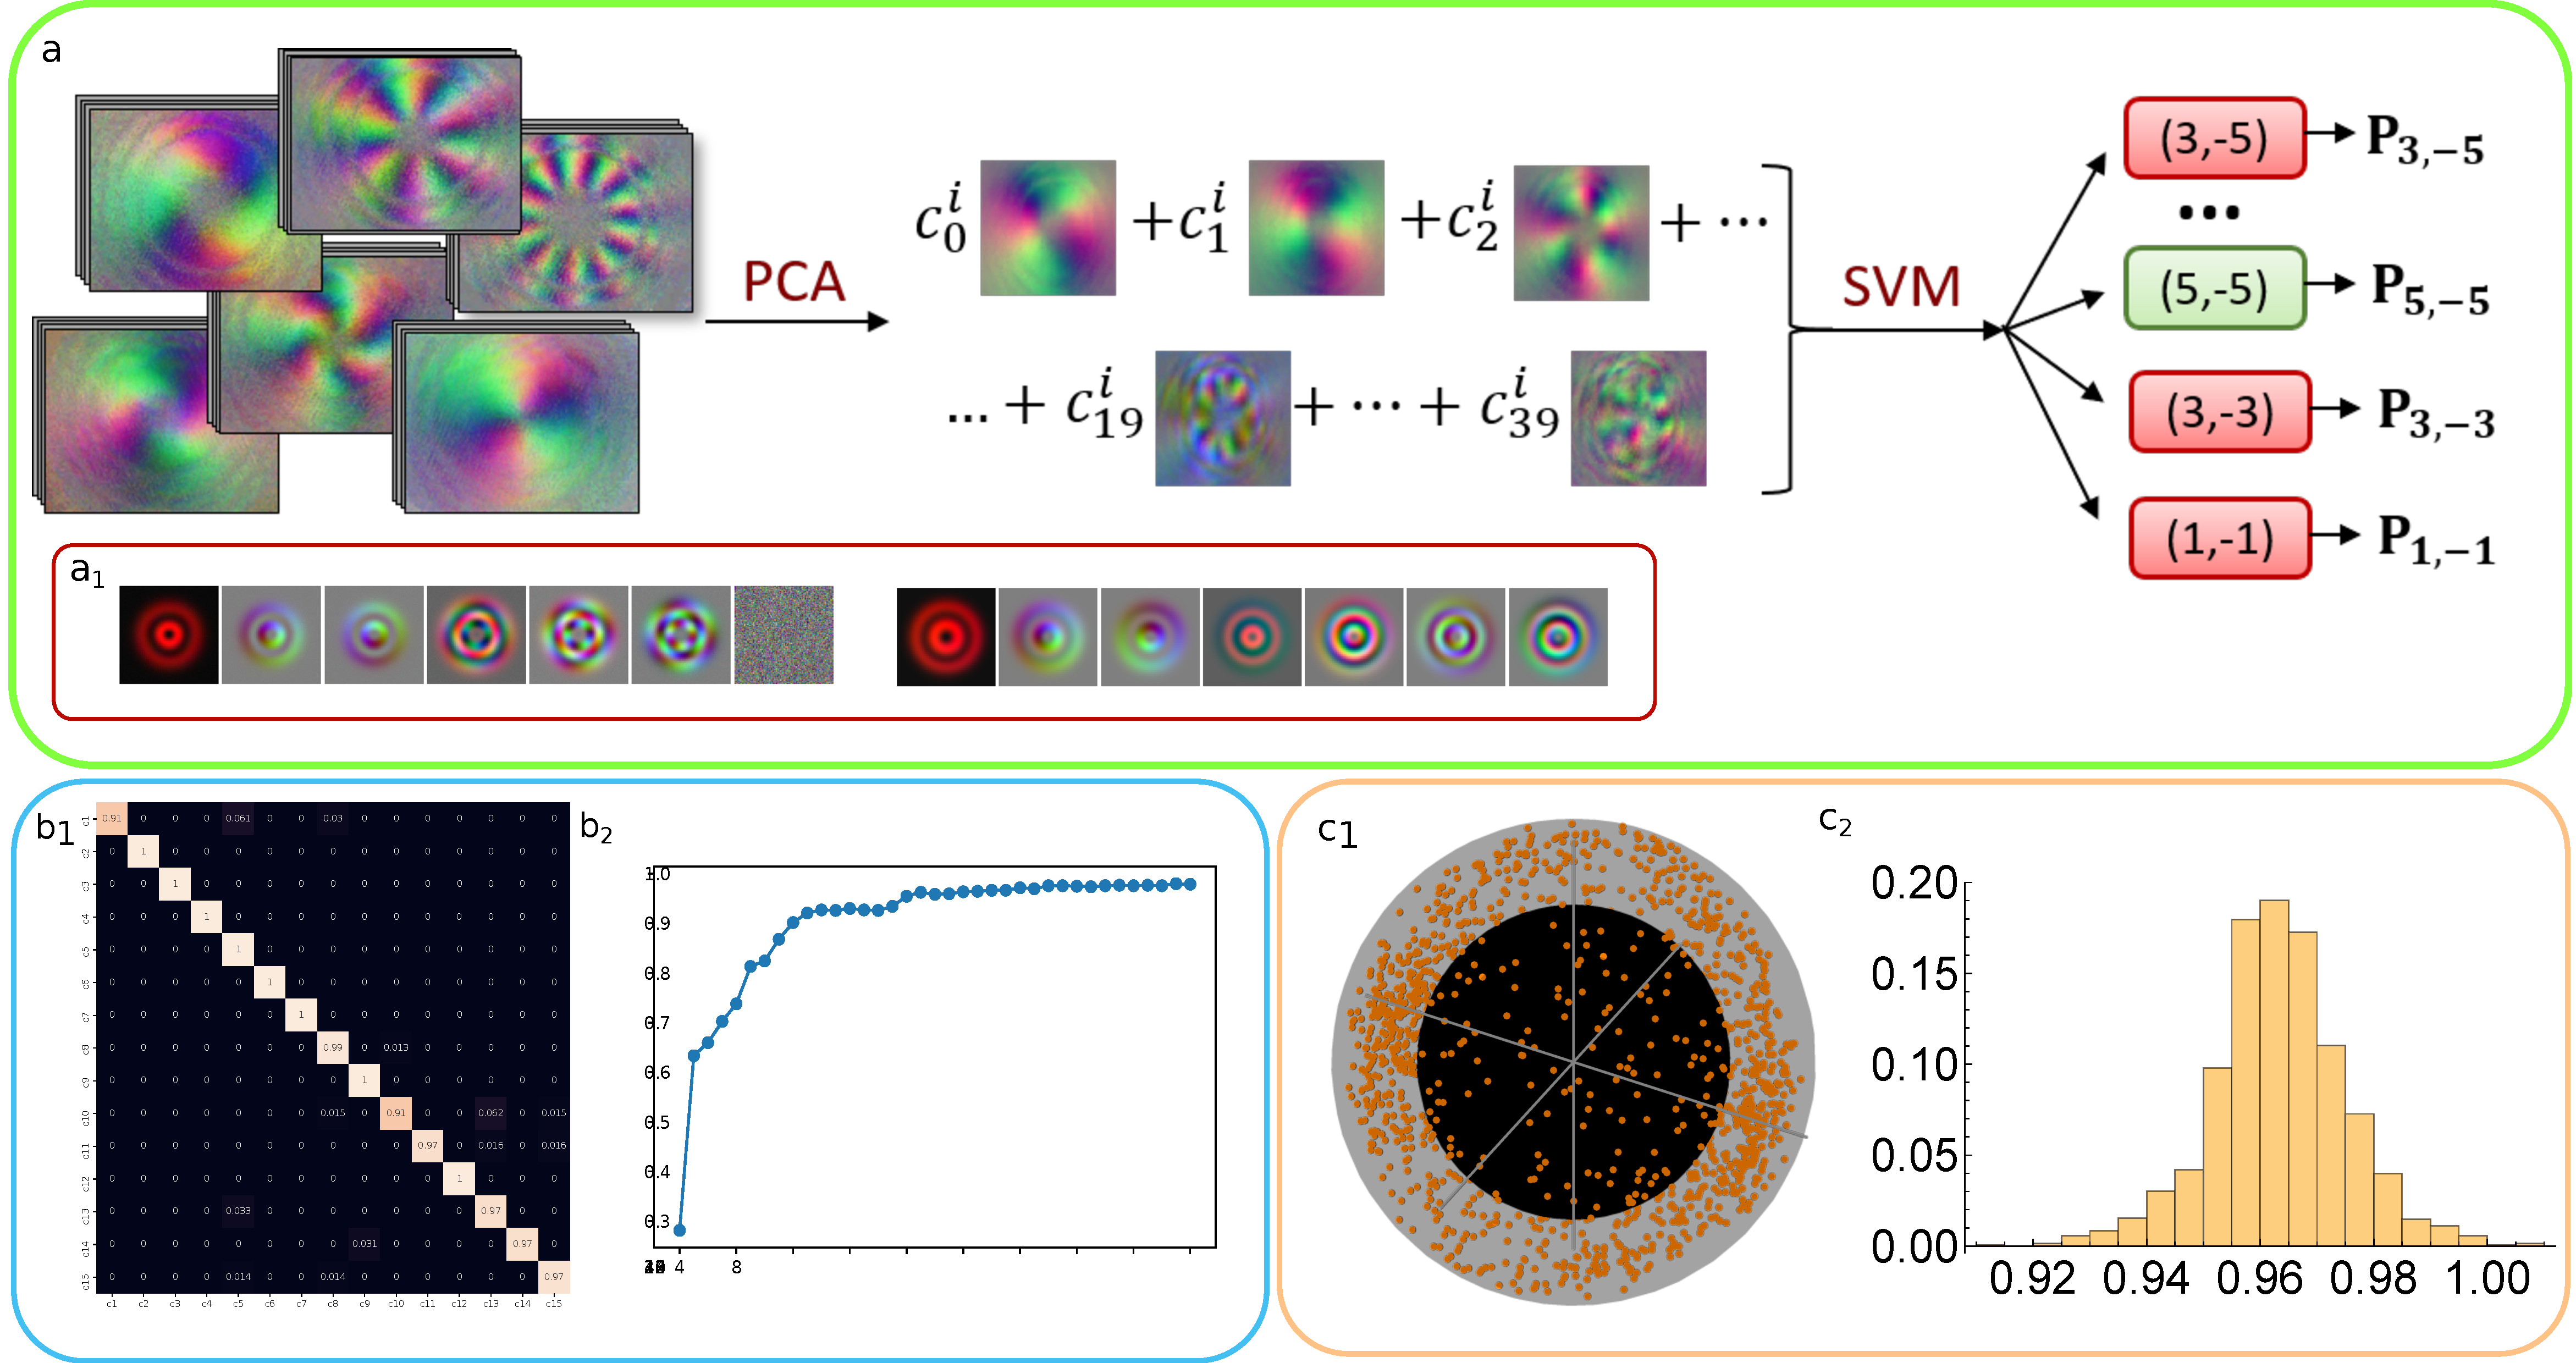
\includegraphics[width=\textwidth]{Figures/quantum-walks/VVBs-PCAResults.pdf}
	\caption{
		% \textbf{Training set on high-order Poincar\'e sphere.}
		% \textbf{\emph{(a)}} Poincar\'e sphere for \acp{VVB} with $|m_{1,2}|=1$.
		% Magenta-coloured parallels (Blue-coloured meridians) mark intervals between consecutive values of $\theta$ ($\phi$). 
	 %    Along a meridian the colours of the pattern vary from the hottest to the coldest ones. Along a parallel the pattern rotates. 
	 %    \textbf{(b)} Comparison between experimental \ac{VVB} with the expected picture for $(\theta, \phi)$ reported below.
	    \textbf{(c)} Histogram of the fidelities between the states retrieved from projection onto the three axes given by \ac{PCA} of the experimental dataset in \textbf{b} and the associated states.
	    %For each  image of the experimental dataset in Fig.~\ref{fig:results_qubit}, we project onto the three principal components given by~\ac{PCA}, and compute the fidelity of the associated state with respect to the one corresponding to the same experimental image. 
	    %We get an average reconstruction fidelity of $\sim0.96$ (standard deviation $\sim0.01$). We find three principal components that carry most of the information.
	    Projection onto such axes and rescaling brings the data (orange points) to the border of a three-dimensional sphere, as shown in the inset. The inner (outer) black (semi-transparent) sphere is added for contrast [radius equal to that of the point with smaller (larger) radius].
	    \textbf{(d)} Average prediction accuracy of a linear \ac{SVM} classifier, trained and tested after applying linear DR on the data, against the number of reduced dimensions $n_c$. 
	    %The average overall accuracy does not improve significantly for more than $\sim25$ dimensions.
	    For each of the 15 classes (cf. Fig.~\ref{fig:resultsCNN}a) in which the experimental dataset was divided, we show in the inset the true-table. %\st{the fraction of images that were classified as belonging to each of the classes}. 
	    %The diagonal represents the ratio of correctly classified images for each label. Each row shows how the images belonging to a given class were classified. 
	}
	\label{fig:PCAresults}
\end{figure}

%\begin{figure*}[ht]
%    \centering
%    \includegraphics[width=0.95\textwidth]{Fig4.pdf}
%    \caption{ \textbf{Principal Component Analysis (PCA) results. a,} %conceptual scheme to classify experimental \ac{VVB} images. First, the %dimension of the dataset is reduced via linear PCA. Then, an SVM %classifier is trained over the reduced representation given by the PCA %to predict the classes of future images of \ac{VVB}s. {\bf b,} %principal components obtained using \ac{PCA} on simulated datasets of %noisy \acp{VVB}. The first row shows the first seven principal %components obtained on the dataset $\mathcal S_1$. The last image shows %that only the first six of such principal components correspond to %non-vanishing singular values. On the other hand, the second row shows %the principal components for the dataset $\mathcal S_2$, and here there %are seven different principal components corresponding to non-vanishing %singular values, as also discussed in the main text. {\bf c,} for each %of the 15 classes in which the experimental dataset was divided, we %show the fraction of images that were classified as belonging to each %of the classes. The diagonal thus represents the ratio of correctly %classified images for each label. Each row shows how the images %belonging to a given class were classified. {\bf d,} average prediction %accuracy of a linear \ac{SVM} classifier, trained and tested after %applying linear dimensionality reduction on the data, as a function of %the number of reduced dimensions $n_c$. The average overall accuracy is %found to not improve significantly using more than $\sim25$ dimensions. %{\bf e,} applying \ac{PCA} to the experimental dataset of %Fig.~\ref{fig:results_qubit}, we find three principal components which %carry the majority of the information. Projecting the data on these %axes %and rescaling them, we find that the data arrange at the border of %a %three-dimensional sphere. Each orange point corresponds to a different %experimental image. The inner black sphere is only added for contrast, and %has radius equal to that of the point with smaller radius. Similarly, the %outer semi-transparent shell encloses the point with larger radius. %\textbf{f,} reconstruction fidelities for the same experimental dataset of %panel {\bf e}. For each experimental image, we project onto the three %principal components given by~\ac{PCA}, and compute the fidelity of the %associated state with respect to the state that we know corresponds to the %same experimental image. The average reconstruction fidelity thus obtained %is $\sim0.96$, with sample standard deviation $\sim0.01$.}
%    \label{fig:PCAresults}
%\end{figure*}

In turn, we can gain information on the generation of the underlying states by only looking at the intensity images captured by a {CCD} camera [cf. Fig.~\ref{fig:qw_poinc_sphere}], and extract the corresponding geometric features of the state space. This resembles a form of \emph{unsupervised} learning, as we gain useful information about the origin of the images without feeding the algorithm with any knowledge of the underlying process.

To demonstrate these ideas we give examples of \ac{PCA} applied to simulated and experimental images. We generate a set of images corresponding to \ac{VVB} states of the form
$c_1\ket{L,m=1}+c_2\ket{R,m=2}$ and put these with images corresponding to states of the form
$c_1\ket{L,m=1}+c_2\ket{R,m=4}$, where the coefficients $c_i$ are sampled uniformly at random from the set of $c_{1,2}\in\mathbb{C}$  such that $|c_1|^2+|c_2|^2=1$.
When \ac{PCA} is applied to the full set of such images, six non-vanishing singular values are found whose associated principal components are shown in Fig.~\ref{fig:class_techniques}c.
This is consistent with the dimension of the subspace  spanned by states of the form $\mathcal S_1=\{c_1\ket1+c_2\ket2, c_1\ket1+c_4\ket4\}$,  as the set of corresponding density matrices is spanned by the four off-diagonal matrices $X^{12,14}, Y^{12,14}$, plus the two diagonal ones $Z^{12,14}$, where $X^{ij}=\ketbra{i}{j}+\ketbra{j}{i}$ is the Pauli $X$ matrix acting on the $(i,j)$ subspace, and similarly for $Y^{ij}$ and $Z^{ij}$.
On the other hand, if the dataset under consideration is generated from states of the form $\mathcal S_2=\{c_1\ket1+c_2\ket2, c_3\ket3+c_4\ket4\}$, \ac{PCA} finds \emph{seven} principal components associated with non-vanishing singular values (see Fig.~\ref{fig:class_techniques}c).
This is consistent with the underlying state space being spanned by the seven traceless Hermitian operators $X^{12,34}, Y^{12,34}, Z^{12,13,14}$.

States such as $c_1\ket{L,m=m_1}+c_2\ket{R,m=m_2}$ can be pictured as lying on a sphere, in the Poincar\'e representation. The associated images thus draw a three-dimensional ellipsoid embedded in the high-dimensional space of intensity images. The application of the technique highlighted above to the dataset of Fig.~\ref{fig:PCAresults}b, shows clearly the three underlying principal components.
Projecting the images onto such principal components, we find that the Poincar\'e sphere is recovered with a good fidelity, as shown in Fig.~\ref{fig:PCAresults}c. This confirms that the method also works under noisy conditions.
Remarkably, once the principal axes are recovered from the data, we can gain an approximate full description of a state from the corresponding experimental intensity pattern, by projecting the data vector onto the first three principal components.
To assess the accuracy of such reconstruction, we compute the fidelity between the density matrix corresponding to the reduced representation found by PCA for any given state, and the corresponding state used to generate the image. As shown in Fig.~\ref{fig:PCAresults}c, the average fidelity between reconstructed and ideal states is $\mathcal F_{\text{avg}}\sim0.96$ (standard deviation $\sim0.01$).



\textit{Classification via SVMs--} We now consider the task of classifying experimental \ac{VVB} images. More precisely, given a dataset of \emph{labelled} \ac{VVB} states, we want to train a classifier to predict the class to which future images of \acp{VVB} belong.
%\rmv{We consider discrete classes defined as specific slices of the state space. More specifically, }
We consider classes of the form $(m_1,m_2)$, as we did for the CNN.
%\rmv{${\cal C}_{m_1, m_2}=\{(\ket{L,m_1}+e^{i\phi}\ket{R,m_2})/\sqrt2\}$ for various phases $\phi$, i.e. balanced superpositions of two different OAM basis states associated to different polarisations.}

We use an \ac{SVM} classifier over the reduced representation given by the \ac{PCA}. Applying the method to an experimental dataset composed of 15 different classes,
%\rmv{ each of the form ${\cal C}_{m_1, m_2}$,}
we get an average $\sim98\%$ accuracy by applying a linear~\ac{SVM} classifier after reducing the dimension of the data to 40 via linear \ac{PCA}.
The~\ac{SVM} was trained on half of the experimental data, with the other half used for testing the resulting accuracy. A breakdown of the classification performance is reported in Fig.~\ref{fig:PCAresults}d, where we detail how the images belonging to each class were classified. %\footnote{We used here a \emph{linear} SVM, instead of a commonly used SVM with RBF kernel, because we found it to perform better: an RBF kernel was found to give, in our case, an average accuracy of only $\sim94\%$.}. %\rmv{We used here a \emph{linear} SVM, instead of a commonly used SVM with RBF kernel, because we found it to perform better: an RBF kernel was found to give, in our case, an average accuracy of only $\sim94\%$.}
In Fig.~\ref{fig:PCAresults}d we show how the average overall accuracy varies with the number of reduced dimensions: $\sim 25$ dimensions are already sufficient  to get good average accuracy.


\textit{Discussion--} We have presented a new approach to the classification of VVBs based on the use of ML techniques. We have demonstrated how the use of inference strategies based on CNNs and PCA (enhanced by SVM) allow for the faithful acquisition of information on a high-dimensional system encoded in the OAM and polarization of a photonic information carrier. While CNN allows for effective classification of VVBs, PCA unveils the possibility to recover the full information of high-dimensional OAM states.
While paving the way to further experimental validations -- possibly in experimental settings that do not rely on optical networks -- we believe our approach to the classification of \ac{VVB}s can be key for a number of relevant tasks in modern photonics, from the design of automatized approaches to the characterization of experimental platforms and experiments, to the provision of potential solutions to OAM demultiplexing in the context of classical and quantum communication and, more in general, for the use of structured light in quantum technologies.
